
\chapter{Background Knowledge}
\label{BackgroundKnowledgeCh}

This chapter will introduce the necessary background knowledge to follow the
theoretical derivations later.

\section{Probability Theory and Statistics}

\subsection{Rules and Theorems}

We here lay out definitions and theorems that we will make use of in the thesis.
For all parts below, assume that $x \in \mathcal{X}$ and $y \in \mathcal{Y}$ are
random variables and $p(x)$ respectively $p(y)$ the probability distributions
of these variables. It will be clear from the context if $x$ is to be
interpreted as a random variable or an observed quantity. We interpret the
integral over $x$ to be a sum over $\mathcal{X}$ if $x$ is discrete and a
regular Lebesgue integral over $\mathcal{X}$ if $x$ is continuous. Then:
\begin{definition}[Unit Volume]
  \label{eq:unit_vol_prob_axiom}
  \begin{equation*}
    \int_{\mathcal{X}}p(x) \dif x = 1
  \end{equation*}
\end{definition}
\begin{definition}[Non-negativity]
  \label{eq:non_neg_of_prob}
  \begin{equation*}
    p(x) \geq 0
  \end{equation*}
\end{definition}

Most manipulations of random variables may be reduced to the following three rules of probability:
\begin{theorem}[Sum Rule]
  \label{eq:sum_rule}
  \begin{equation*}
    p(x) = \int_{\mathcal{Y}}p(x, y) \dif y
  \end{equation*}
\end{theorem}
\begin{theorem}[Product Rule]
  \label{eq:product_theorem}
  \begin{equation*}
    p(x, y) = p(y | x)p(x)
  \end{equation*}
\end{theorem}
\begin{theorem}[Bayes Rule]
  \label{eq:Bayes_theorem}
  \begin{equation*}
    p(y | x) = \frac{p(x | y)p(y)}{p(x)}
  \end{equation*}
\end{theorem}

Two very important operations involving probabilities of random variables are
those of \textit{Expectation} and \textit{Covariance}.
\begin{definition}[Expectation]
  \label{eq:expectation}
  Let $f : \mathcal{X} \to \mathbb{R}$, then
  \begin{equation*}
    \E_x[f] = \int_{\mathcal{X}} f(x) p(x) \dif x
  \end{equation*}
\end{definition}
\begin{definition}[Covariance]
  \label{eq:covariance}
  \begin{equation*}
    \Cov(x, y) = \E_{xy}[(x - \E_x[x])(y - \E_y[y])]
  \end{equation*}
\end{definition}
The variance operator is straightforwardly defined:
\begin{definition}[Variance]
  \label{eq:variance}
  \begin{equation*}
    \Var(x) = \Cov(x, x)
  \end{equation*}
\end{definition}

The generalisation of expectation from $f: \mathcal{X} \to \mathbb{R}$ to $f: \mathcal{X} \to
\mathbb{R}^D$ is straightforward. If $\bm{f} =
f(x)$ then:
\begin{equation*}
  \E_x
  \begin{bmatrix}
    \bm{f}_1 \\
    \vdots \\
    \bm{f}_D \\
  \end{bmatrix} =
  \begin{bmatrix}
    \E_x \bm{f}_1 \\
    \vdots \\
    \E_x \bm{f}_D \\
  \end{bmatrix}
\end{equation*}
similarly $\Cov(\bm{f})$ is a $D \times D$-dimensional matrix where
$\Cov(\bm{f})_{i,j} = \Cov(\bm{f}_i,
\bm{f}_j)$\cite{Bishop:2006, Barber:2012:BRM:2207809}.

\subsection{The Gaussian Distribution}
For a $D$-dimensional random vector $\bm{x}$, the multivariate Gaussian
distribution takes the form
\begin{equation}
  \label{eq:Gaussian_dist}
  \mathcal{N}(\bm{x} | \bm{\mu}, \bm{\Sigma}) = \frac{1}{(2\pi)^{D/2}}\frac{1}{|\bm{\Sigma}|^{1/2}}\exp\left( -\frac{1}{2}(\bm{x} - \bm{\mu})^T\bm{\Sigma}^{-1}(\bm{x} - \bm{\mu})\right),
\end{equation}
where $\bm{\mu}$ is a $D$-dimensional mean vector, $\bm{\Sigma}$ is a $D \times
D$ dimensional positive definite covariance matrix and $|\bm{\Sigma}|$ denotes
the determinant of $\bm{\Sigma}$. It is straightforward to show that these
parameters correspond to the mean and covariance as defined in
\ref{eq:expectation} and \ref{eq:covariance} \cite{Barber:2012:BRM:2207809}.

The Gaussian distribution can be seen as a unit $D$-dimensional cube which is
translated, sheared and rotated, giving rise to the fact that we can write any
Gaussianly distributed random variable $\bm{x} \sim \mathcal{N}(\bm{x} |
\bm{\mu}, \bm{\Sigma})$ as a linear combination of a unit Gaussian random
variable $\bm{z} \sim \mathcal{N}(\bm{x} | \bm{0}, \bm{I})$. If
we let $\bm{\Lambda} \bm{\Lambda}^{\top} = \bm{\Sigma}$ be the Cholesky
decomposition \cite[p.~100-102]{Press:2007:NRE:1403886} of $\bm{\Sigma}$, then we
also have that
\begin{equation}
  \label{eq:sample_x}
  \bm{x} = \bm{\mu} + \bm{\Lambda}\bm{z},
\end{equation}
where the equality is in terms of distribution. If we further assume that
$\bm{x}$ is parametrised by $\bm{\mu}$ and $\bm{\Sigma}$ such that $\bm{\Sigma}$
is diagonal positive definite with diagonal $\bm{\sigma}^2$, and furthermore
$\bm{\sigma} = \sqrt{\bm{\sigma}^2}$ where the square root is taken elementwise, then this means that if we want to
sample a random variable $\bm{x}$ with diagonal covariance structure, we
can do this by sampling a unit normal $\bm{z}$ which we then transform, which
may be expressed as
\begin{equation}
  \label{eq:sample_x_diag_covariance}
  \bm{x} = \bm{\mu} + \bm{\sigma} \odot \bm{z} \sim \mathcal{N}(\bm{\mu}, \bm{\sigma}^2),
\end{equation}
where we define a vector $\bm{\sigma}^2$ as the covariance matrix $\bm{\Sigma}$ to
mean that $\bm{\Sigma}$ is diagonal positive definite with diagonal
$\bm{\sigma}^2$. In this case we have used the elementwise product operator
$\odot$ which in general takes two matrices $\bm{A}, \bm{B}$ such that $(\bm{A}
\odot \bm{B})_{ij} = \bm{A}_{ij} \bm{B}_{ij}$.

As the Gaussian distribution is part of the exponential
family \cite{Barber:2012:BRM:2207809}, the density of the joint distribution of
iid\footnote{Identically, Independently Distributed} Gaussian variables are themselves Gaussian distributed where the natural
parameters of this joint distribution is the sum of the natural parameters of
each random variable in the joint. In particular for the Gaussian distribution,
this means that if we have a collection of iid gaussian random variables
$\{\bm{x}_i\}_i^n$, such that $\bm{x}_i \sim \mathcal{N}(\bm{x}_i | \bm{\mu}_i,
\bm{\Sigma}_{i})$, then the joint can be found to be Gaussian distributed as
\begin{equation*}
  \mathcal{N}(\bm{\mu}, \bm{\Sigma}),
\end{equation*}
where
\begin{align}
  \bm{\Sigma} & = \left( \sum_i^n \bm{\Sigma}_i^{-1} \right)^{-1} \label{eq:joint_indep_normal_covariance}\\ 
  \bm{\mu} & = \bm{\Sigma}\left( \sum_i^n \bm{\Sigma}^{-1} \bm{\mu}_i \right) \label{eq:joint_indep_normal_mean}.
\end{align}\cite[p.~78-84]{Bishop:2006}

For example in the case of two independent random variables distributed
according to the form as laid out in \eqref{eq:sample_x_diag_covariance}, $\bm{x} \sim
\mathcal{N}(\bm{\mu}_{\bm{x}}, \bm{\sigma}^2_{\bm{x}})$
and $\bm{y} \sim \mathcal{N}(\bm{\mu}_{\bm{y}}, \bm{\sigma}^2_{\bm{y}})$, we have that the resulting distribution $p(\bm{x}, \bm{y}) =
p(\bm{x})p(\bm{y})$ is distributed such that
\begin{equation*}
  p(\bm{x}, \bm{y}) = \mathcal{N}(\bm{\mu}_{\bm{x}, \bm{y}}, \bm{\sigma}^2_{\bm{x}, \bm{y}})
\end{equation*}
where
\begin{align}
  \bm{\sigma}_{\bm{x}, \bm{y}} & = \frac{1}{(\bm{\sigma}_{\bm{x}}^2)^{-1} + (\bm{\sigma}^2_{\bm{y}})^{-1}} \label{eq:joint_indep_normal_covariance_diag}\\
  \bm{\mu}_{\bm{x}, \bm{y}} & = \frac{(\bm{\sigma}^2_{\bm{x}})^{-1} \odot \bm{\mu}_{\bm{x}} + (\bm{\sigma}^2_{\bm{y}})^{-1} \odot \bm{\mu}_{\bm{y}}}{(\bm{\sigma}^2_{\bm{x}})^{-1} + (\bm{\sigma}^2_{\bm{y}})^{-1}} \label{eq:joint_indep_normal_mean_diag}
\end{align}
with the inverse and division operators being done elementwise. This can be
derived in a straightforward manner by using the precision matrix instead of the
covariance matrix.

\subsection{Maximum Likelihood Estimation}

Assume we have a model $\mathcal{M}$ parametrised by $\bm{\theta}$ constrained
to live in the parameter space $\bm{\Theta}$. Given data $\mathcal{D} = \{\bm{x}_i\}_{i=1}^n$ we want
to be able to fit the parameters $\bm{\theta}$ such that the model generalise to
unseen data.

We define the likelihood function using the common assumption of iid datapoints
\begin{equation}
  \label{eq:likelihood}
  \mathcal{L}(\bm{\theta} | \mathcal{D}) = p(\bm{x}_1, \dots, \bm{x}_n | \bm{\theta}) = \prod_i^n p(\bm{x}_i | \bm{\theta}).
\end{equation}
The MLE of of the parameters of the model is then defined to be
\begin{equation}
  \label{eq:MLE}
  \hat{\bm{\theta}}_{ML} = \argmax_{\bm{\theta} \in \bm{\Theta}}\mathcal{L}(\bm{\theta} | \mathcal{D}).
\end{equation}

While the original MLE is defined in terms of the likelihood function
$\mathcal{L}(\bm{\theta}| \mathcal{D})$, it's often more practical to work with
the logarithm of this function, the log-likelihood function $\ell(\bm{\theta} |
\mathcal{D})$. Using the log-likelihood we transform this product into a form involving sums
\begin{equation}
  \label{eq:loglikelihood}
  \ell(\bm{\theta} | \mathcal{D}) = \log \mathcal{L}(\bm{\theta} | \mathcal{D}) = \sum_i^n \log p(\bm{x}_i).
\end{equation} \cite{CaseBerg:01}

Besides from simplifying notation and calculation, the log-likelihood has the added benefit of
reducing the risk of arithmetic underflow due to the small magnitude of
individual probabilities. In models with long dependency such as language
models, working in the log-space is needed to enable computation efficiently and
robustly.

\section{Deep Learning}
The field of NLP were originally dominated by older machine learning
techniques utilising linear models trained over very high-dimensional and sparse
feature vectors. Recently the field has switched over to neural networks over
dense inputs using word embeddings \cite[p.~1 - 2]{goldberg2015primer}.

Neural networks may be seen from many angles, but from a mathematical point of
view a neural network parametrised by parameters (weights) $\bm{\theta}$
specifies a non-linear functional relationship between the input to the network $\bm{x}$
and the output $\bm{y}$. As such a neural network architecture with unspecified parameters
$\bm{\theta}$ in a parameter space $\Theta$ specifies a set of functions
\cite{Bishop:2006}. It has been shown that this set of functions of several
architectures are universal approximators and thus are able to approximate
continuous functions on compact subsets of $\mathbb{R}^m$ \cite{Hornik:1989:MFN:70405.70408, Cybenko1989univapprox},
justifying their use theoretically.

\subsection{Multilayer Perceptron}
Multilayer Perceptrons (MLP's) are neural networks represented by functional composition, where each
function is interpreted as a layer of the network. The original MLP can be defined in
terms of a recurrence relation such that if we have input vectors of the form $\bm{x} \in
\mathbb{R}^{d_{in}}$ and output vectors of the form $\bm{y} \in
\mathbb{R}^{d_{out}}$ and $\sigma_i( \cdot )$ represents an arbitrary activation
function (also called nonlinearity), then an MLP with $L$ layers have the functional form
\begin{equation}
  f(\bm{x} | \bm{\theta}) = \sigma_L(\bm{W}_L \bm{z}_{L-1} + \bm{b}_{L})
\end{equation}
where for any $l \in \{2, \dots, L-1\}$
\begin{equation}
    \bm{z}_l = \sigma_l(\bm{W}_l \bm{z}_{l-1} + \bm{b}_l)
\end{equation}
with base case
\begin{equation}
  \bm{z}_1 = \sigma_1(\bm{W}_1 \bm{x} + \bm{b}_1).
\end{equation} \cite{BarberAppliedML}

$\bm{W}_l$ and $\bm{b}_l$ may be of any dimension as long as it is dimensionally consistent
with the input and output of the previous and next layers and conform to the
original input and output dimensions. In this case we have that the parameters
of the network are all of the biases and weights for the layers, $\bm{\theta} =
\{(\bm{W}_l, \bm{b}_l)\}_{l = 1}^L$.

Activation functions generally are monotonically increasing function mapping real
numbers to some interval. Activation functions which will be useful to us are
\begin{description}
\item[Sigmoid]
  \begin{equation}
    \label{eq:sigmoid}
    \sigma(x) = \frac{1}{1 + \exp(-x)}
  \end{equation}
  The sigmoid activation function maps any real number to a value in $(0, 1)$.
\item[Hyperbolic tangent]
  \begin{equation}
    \label{eq:tanh}
    \tanh(x) = \frac{2}{1 + \exp(-2x)} - 1 = 2 \sigma(2x) - 1
  \end{equation}
\item[SELU]
  Scaled Exponential Linear Units \cite{DBLP:journals/corr/KlambauerUMH17} have the form
  \begin{equation}
    \label{eq:SELU}
    \text{selu}(x) = \lambda
    \begin{cases}
      x \quad\text{if $x > 0$} \\
      \alpha(\exp(x) - 1) \quad \text{if $x \leq 0$}
    \end{cases}
  \end{equation}
\item[Softmax]
  The Softmax is a mapping from an input space $\mathbb{R}^{d_{in}}$ to an output
  space $\mathbb{R}^{d_{out}}$, the form given by
  \begin{equation}
    \label{eq:softmax}
    \text{softmax}(\bm{z})_i = \frac{\exp(z_i)}{\sum_{k=1}^{d_{out}}\exp(z_k)} \quad \text{where} \quad i \in \{1, \dots, d_{out}\}
  \end{equation}
  Since it is normalized it is a natural candidate for defining categorical
  distributions \cite{Barber:2012:BRM:2207809} and we will use it for this
  purpose in our models.
\end{description}

\subsection{Recurrent Neural Networks}

RNN's have traditionally been the neural network architecture of choice for NLP
due to it being able to handle long-term dependencies well \cite{KarpathyRNN}. We use the LSTM cell in our RNN which handles the vanishing gradient problem in
neural networks. For in depth treatment of the architecture with respect to NLP
see \cite{Hochreiter:1997:LSM:1246443.1246450, sundermeyer2012lstm}.

\subsection{Convolutional Neural Networks}
\label{ch:WaveNet}
The CNN we will use will be highly specialised for our case. We use the WaveNet
as laid out in the paper by DeepMind \cite{DBLP:journals/corr/OordDZSVGKSK16}.
We will use the condition form.

Conditional WaveNet works on data of the form of vectors, $\bm{x} = (x_1, \dots,
x_L)^T$, conditioning on a vector $\bm{z}$, were we describe the distribution as
\begin{equation*}
p(\bm{x} | \bm{z}) = \prod_{l=1}^L p(x_l| x_1, \dots, x_{l-1}, \bm{z}),
\end{equation*}
the form common in NLP. The output of the model has the same
time dimensionality as the input, meaning that the model has the ability to
output a categorical distribution over the next value $x_l$ with a softmax
layer. In our case this is a parametrisation of the output probability at point
$l$.

WaveNet uses dilated convolutions, a type of convolution where the filter is applied
to an area larger than its length by only considering input values such that at
each step you skip $k$ inputs, where $k$ is the dilation. Stacking layers and
using dilations that increase exponentially with the depth of the layer, it is
possible to get a receptive field which grows exponentially with the depth of
the network \cite{DBLP:journals/corr/OordDZSVGKSK16}.

\begin{figure}[H]
  \centering
  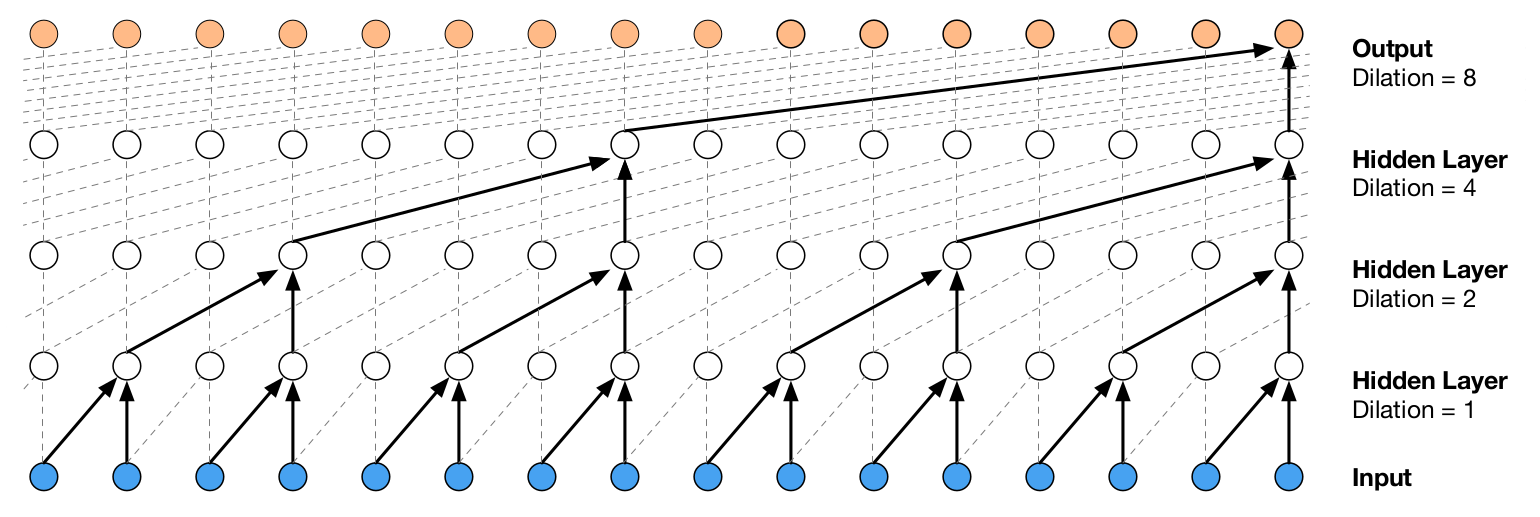
\includegraphics[width=1.0\textwidth]{wavenet_dilated_convolutions}
  \caption{Dilated Convolutions in WaveNet \cite{DBLP:journals/corr/OordDZSVGKSK16}}
  \label{fig:wavenet_dilated_convolutions}
\end{figure}

We use residual connections in order to speed up training.

\section{Natural Language Processing}

Humans use natural language every day to convey concepts and abstractions to each
other in an efficient manner. Compared to formal languages found in
mathematics and programming, the natural languages we use are often
ambiguous systems filled with rules and exceptions \cite{Rosenfeld00twodecades,
  sep-computational-linguistics}.

We will here go through the necessary theory for understanding the neural language model we
will build.

\subsection{Language model}
We define a sentence to be a vector of words $\bm{x}_{1:L} = (\mathsf{x}_1, \dots,
\mathsf{x}_L)^{\top}$ such that each word is an atomic element $\mathsf{x}_i \in
V$, where $V$ is the dictionary of words in our language. Repeated use of the
product rule laid out in \eqref{eq:product_theorem} enables us to rewrite the probability
of a sentence in terms of how it is composed of words
\begin{equation}
  \label{eq:conditional_language_probability}
  P(\bm{x}_{1:L}) = \prod_{l = 1}^LP(\mathsf{x}_l | \mathsf{x}_1, \dots, \mathsf{x}_{l-1})
\end{equation}
where $\mathsf{x}_l$ is the $l$'th word of the sentence
$\bm{x}_{1:L}$ \cite{Bengio:2003:NPL:944919.944966}.

This form of the probability of a sentence lays bare how the words in a sentence
relate to previously occurred words within the same sentence. We will assume
that all sentences in the dataset $\mathcal{D} = \{\bm{x}^n\}_{n=1}^N$ are iid
which enables us to express the log-likelihood in the form of equation
\eqref{eq:loglikelihood}.

\subsection{Word embeddings}
Breaking down sentences at a word level and processing them into a form that
encodes information efficiently is a problem which has gained notorious
recognition \cite{DBLP:journals/corr/abs-1301-3781}, leading to algorithms such
as word2vec \cite{Mikolov:2013:DRW:2999792.2999959} and
Glove \cite{Pennington14glove:global}. However, these techniques work less well
in a neural network setting where instead the preferred technique is to find the
best embeddings jointly with the parameters of the model using backpropagation \cite[p.~5-7]{goldberg2015primer}.

A straightforward way to represent the various words of the dictionary is as
one-hot-encoded vectors such that a word $\mathsf{x} \in V$, where the size of
$V$ is $|V|$, with an index $i$ given by its place in the dictionary sorted
alphabetically in descending order will have the vector representation
\begin{equation}
  \label{eq:one_hot_encoding}
  \text{onehot}(\mathsf{x}) =
  \begin{bmatrix}
    0 \\
    \vdots \\
    0 \\
    1 \\
    0 \\
    \vdots \\
    0
  \end{bmatrix}
\end{equation}
such that $\text{onehot}(\mathsf{x})_j = \delta_{ij}$ \cite[p.~6]{goldberg2015primer}.
While this is a form conceptually easy to understand, it fails to account for the
curse of dimensionality as the size of the vocabulary grows large in practice
and the fact that the cosine similarity of two words $\mathsf{x}_1,
\mathsf{x}_2 \in V$ is zero unless they are the same word,
\begin{equation}
  \label{eq:cosine_similarity}
  \cos_{similarity}(\text{onehot}(\mathsf{x}_1), \text{onehot}(\mathsf{x}_2)) = \delta_{\mathsf{x}_1 \mathsf{x}_2}.
\end{equation} This means that no meaning is embedded in the vector space
except for the location in the sorted dictionary. Instead we would like to
associate each word in the vocabulary with a distributed \textit{word feature
  vector}, that is a dense, real-valued vector in $\mathbb{R}^m$ where $m$ is the
dimension of our embedding space. After training this embedding jointly with the
parameters of the network, words which share similarities such as \texttt{Dog,
  Puppy} would have a higher similarity score than with an unrelated concepts such as
\texttt{Dog, Bulwark} \cite{Bengio:2003:NPL:944919.944966}.

We may represent this in a mathematical form by trying to find a linear map $C$
from any element $\mathsf{x} \in V$ such that $C(\mathsf{x}) \in \mathbb{R}^E$,
where $E$ is the embedding dimension.
Using the canonical basis of the Euclidean space, we can express this
linear map in terms of a matrix $\bm{C} \in \mathbb{R}^{E \times |V|}$, thus the
word feature vector of the learned embedding can be represented by the matrix
multiplication $\bm{C} \text{onehot}(\mathsf{x})$.

\subsection{Neural machine translation}
For a long time the dominant paradigm within machine translation was to use
phrase based machine translation systems \cite{Koehn:2003:SPT:1073445.1073462,
  Koehn:2007:MOS:1557769.1557821}, recently however, modelling the word or
character level directly with neural networks has overtaken phrase based
translation systems \cite{wolk_neural-based_2015, wu_googles_2016}. These
systems are called Neural Machine Translation.

Most NMT models work in terms of an encoder-decoder architecture where the
encoder extracts a fixed length representation $\bm{c}$, often called a context
vector, from a variable length input sentence $\bm{x} \in \lang{X}$, and the
decoder uses this representation to generate a correct translation $\bm{y} \in
\lang{Y}$ from this representation \cite{cho_properties_2014} as can be seen in
Figure ~\ref{fig:encoder_decoder}.

\begin{figure}[H]
  \includestandalone[width=\textwidth]{./scripts/tikz_code/encoder_decoder}% 
    \caption{Encoder decoder schematic}
  \label{fig:encoder_decoder}
\end{figure}

Our model builds on this paradigm but instead of considering context vectors
$\bm{c}$ we instead consider distributions over a latent vector $\bm{z}$ which
in theory should give the model a greater expressive power since the
distribution relays more knowledge than a direct point estimate.

\section{Optimization}

Most parts of machine learning reduces to optimization of a loss function. While
optimisation of convex problems are well-understood there has been considerable
interest in ways to optimize non-convex loss functions such as those used
traditionally in deep learning.

While theoretical results are lacking, there has been substantial
advances in various optimisation techniques fit to attack the highly non-linear,
non-convex and high-dimensional optimization problems of learning in deep
models, particularly from Stochastic Gradient Descent and its friends. This has
led to numerous gradient descent-like algorithms used machine learning
\cite{Ruder17}.

\subsection{Stochastic Gradient Descent}

For a normal probabilistic machine learning problem, we have data $\mathcal{D}$
that we try to model with a model $\mathcal{M}$ parametrised by parameters
$\bm{\theta} \in \Theta$. The optimization problem in our case can be recast
as an effort to find the parameters $\bm{\theta}_{ML}$ that maximizes the
log-likelihood function \eqref{eq:loglikelihood} or equally minimizes the
negative log-likelihood.

Gradient descent takes steps in the direction of the gradient, which also is the
direction of steepest descent. If we let $\mathcal{D} = \{\bm{x}_i\}_{i = 1}^n$
be our set of sentences and $-\ell$ be the negative log-likelihood that we are
trying to minimize then the updates are of the form
\begin{equation}
  \label{eq:GD_update}
  \bm{\theta}_{t + 1} = \bm{\theta}_t - \gamma \frac{1}{n} \sum_{i = 1}^n \nabla_{\bm{\theta}} (-\ell(\bm{\theta}| \bm{x}_i)),
\end{equation}
where $\gamma$ is the learning rate of the algorithm.

Stochastic Gradient Descent is a similar algorithm to GD that instead of
calculating the gradient with respect to the whole dataset calculates an
approximate gradient, as it only takes a subset of the data into account at each
update. If we let $I_t$ be a random subset of the indices of $\{(\bm{x}_n)_{n=1}^N\}$ of size $m$ then SGD does the following update
\begin{equation}
  \label{eq:SGD_update}
  \bm{\theta}_{t + 1} = \bm{\theta}_t - \gamma \frac{1}{m} \sum_{i \in I_t} \nabla_{\bm{\theta}} (-\ell(\bm{\theta}| \bm{x}_i))
\end{equation}\cite{series/lncs/Bottou12}\cite[p.~240]{Bishop:2006}.

\subsection{ADAM}
SGD has found widespread use within the machine learning community due to strong
experimental results and ease of use, especially in deep learning. However there
are notable alternatives that try to improve on SGD such as
RMSProp\cite{Tieleman2012} and AdaGrad\cite{Duchi:EECS-2010-24}.

Adam takes inspiration from RMSProp and AdaGrad. Technically, Adam keeps an
exponential running average of the first and second order statistics of the
gradient, using these to calculate an adaptive learning rate.

As laid out in the original paper by Kingma et al. \cite{kingma_adam:_2014}, ADAM operates on a
stochastic objective function $f_t(\bm{\theta})$, where $t$ denotes the time
step, similarly $g_t = \nabla_{\bm{\theta}}f_t(\bm{\theta})$. $m_t$ and $v_t$ denotes the first and second order moments of
the gradients, however, these are biased and are corrected in the algorithm.
The whole algorithm is as follows.
\begin{algorithm}[H]
  \caption{ADAM}\label{ADAM}
  \begin{algorithmic}[1]
    \Require $\alpha$: Stepsize
    \Require $\beta_1, \beta_2 \in [0, 1)$: Exponential decay rates of the moment estimates
    \Require $f(\bm{\theta})$: Stochastic objective function with parameters
    $\bm{\theta}$
    \Require $\bm{\theta}_0$: Initial parameter vector
    \State $m_0 \gets 0$ (Initialize $1^{\text{st}}$ moment vector)
    \State $v_0 \gets 0$ (Initialize $2^{\text{nd}}$ moment vector)
    \State $t \gets 0$ (Initialize timestep)
    \While{$\bm{\theta}_t$ not converged}
    \State $t \gets t + 1$
    \State $g_t \gets \nabla_{\bm{\theta}}f_t(\bm{\theta}_{t-1})$ (get gradients w.r.t stochastic objective at timestep $t$)
    \State $m_t \gets \beta_1 \cdot m_{t-1} + (1 - \beta_1) \cdot g_t$ (Update biased first moment estimate)
    \State $v_t \gets \beta_2 \cdot v_{t-1} + (1 - \beta_2) \cdot g^2_t$ (Update biased second raw moment estimate)
    \State $\hat{m}_1 \gets m_t / (1 - \beta^t_1)$ (Compute bias-corrected first moment estimate)
    \State $\hat{v}_1 \gets v_t / (1 - \beta^t_2)$ (Compute bias-corrected second raw moment estimate)
    \State $\bm{\theta}_t \gets \bm{\theta}_{t-1} - \alpha \cdot \hat{m}_i/(\sqrt{\hat{v}_t} + \epsilon)$ (Update parameters)
    \EndWhile
    \Return $\bm{\theta}_t$ (Resulting parameters)
  \end{algorithmic}
  \caption{The ADAM algorithm}
\end{algorithm}

Experimentally Adam has shown very good results on training various deep
learning models such as MLP's, CNN's and RNN's \cite{kingma_adam:_2014}, we will
use it to train all our models.

\subsection{Automatic Differentiation}
\label{ch:autodiff}
The AutoDiff framework is a general theory for efficiently
calculating gradients with respect to a loss function in general computational graphs.
It includes the famed backpropagation \cite{Bishop:2006,
  Rumelhart:1986:LIR:104279.104293} algorithm as a special instance.

In machine learning we most often deal with many-to-one mappings with a
high-dimensional input $\bm{x}$ to a scalar output in the form of a loss. In
terms of machine learning models, AutoDiff takes a loss function
$L(\bm{\theta})$ and returns an exact value up to machine accuracy for the
gradient $\nabla_{\bm{\theta}} L(\bm{\theta}) \vert_{\hat{\bm{\theta}}}$. There are
two different modes of AutoDiff, forward and reverse, although in practice
reverse is preferred.

Reverse mode AutoDiff is efficient in the way that calculating the gradient of
$L(\bm{\theta})$ is guaranteed to take at most 5 times the time it takes to
compute $L(\bm{\theta})$ \cite{Barber15deeplearning:}, enabling neural network
libraries to calculate the gradients needed for optimization algorithms such as
SGD and ADAM in a swift and automatic manner.
